% fig01_disagreement.tex — headline figure, pgfplots standalone (no python dep).
% Cohen's d of (planning depth-ladder) minus (greedy), verbatim from
% .verdicts/1012_bigphi_faithful_larger_n/h1012.txt:
%   n=4: big-Phi d=-1.83  faithful d=+5.18
%   n=5: big-Phi d=-2.28  faithful d=+4.65
\documentclass[border=4pt]{standalone}
\usepackage{pgfplots}
\pgfplotsset{compat=1.18}
\usepackage{amsmath}
\begin{document}
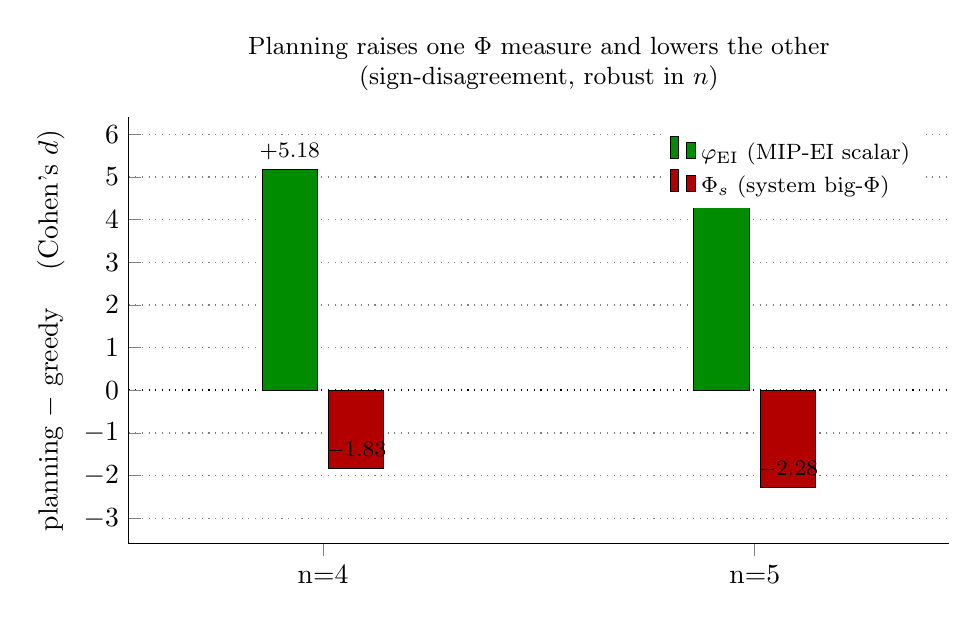
\begin{tikzpicture}
\begin{axis}[
    width=12cm, height=7cm,
    ybar=4pt,
    bar width=20pt,
    enlarge x limits=0.45,
    ymin=-3.6, ymax=6.4,
    ytick={-3,-2,-1,0,1,2,3,4,5,6},
    axis lines*=left,
    axis line style={-},
    extra y ticks=0, extra y tick labels={}, extra y tick style={grid=major, grid style={black, thick}},
    ymajorgrids=true, grid style={dotted, gray},
    symbolic x coords={n=4, n=5},
    xtick=data,
    ylabel={planning $-$ greedy \quad (Cohen's $d$)},
    nodes near coords,
    nodes near coords style={font=\footnotesize\bfseries, /pgf/number format/print sign=true, /pgf/number format/fixed, /pgf/number format/fixed zerofill, /pgf/number format/precision=2},
    every node near coord/.append style={anchor=south},
    legend style={at={(0.97,0.97)}, anchor=north east, draw=none, font=\footnotesize},
    legend cell align=left,
    title style={font=\small, align=center},
    title={Planning raises one $\Phi$ measure and lowers the other\\(sign-disagreement, robust in $n$)},
]
\addplot[fill=green!55!black, draw=black] coordinates {(n=4, 5.18) (n=5, 4.65)};
\addplot[fill=red!70!black, draw=black]   coordinates {(n=4, -1.83) (n=5, -2.28)};
\legend{$\varphi_{\mathrm{EI}}$ (MIP-EI scalar), $\Phi_s$ (system big-$\Phi$)}
\end{axis}
\end{tikzpicture}
\end{document}
